% !TEX TS-program = pdflatex
% !TEX encoding = UTF-8 Unicode
\documentclass[border=0mm]{standalone}
% packages
\usepackage{tikz}
\usetikzlibrary{patterns}
\usepackage{amsmath,amssymb}
\usepackage{bm}
\usepackage{pgfplots}
\pgfplotsset{compat=1.15}
% start document
\begin{document}
% generated by ROOT (CERN)
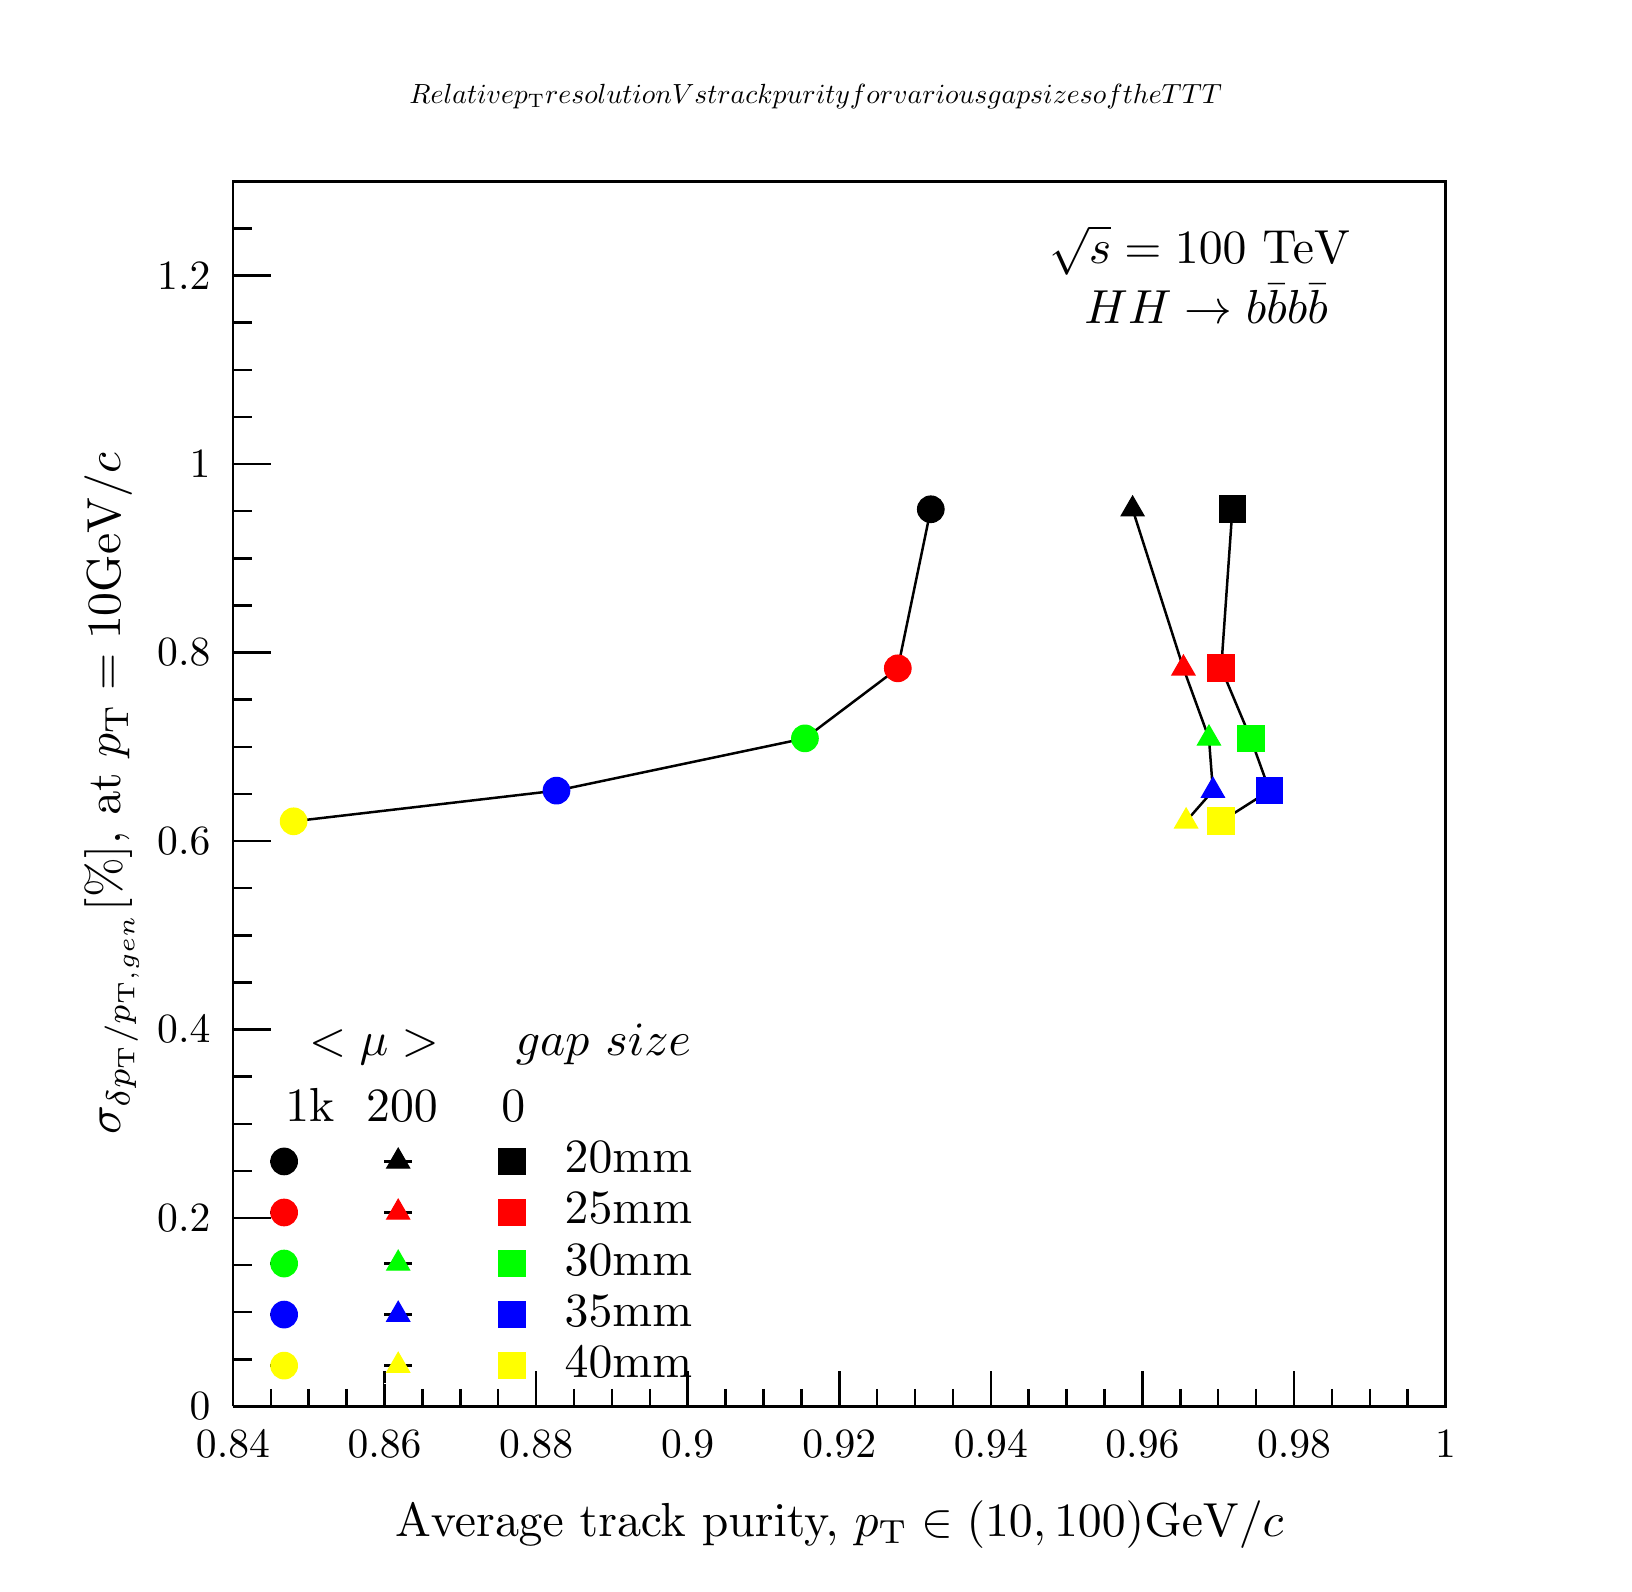
\begin{tikzpicture}
\pgfdeclareplotmark{cross} {
\pgfpathmoveto{\pgfpoint{-0.3\pgfplotmarksize}{\pgfplotmarksize}}
\pgfpathlineto{\pgfpoint{+0.3\pgfplotmarksize}{\pgfplotmarksize}}
\pgfpathlineto{\pgfpoint{+0.3\pgfplotmarksize}{0.3\pgfplotmarksize}}
\pgfpathlineto{\pgfpoint{+1\pgfplotmarksize}{0.3\pgfplotmarksize}}
\pgfpathlineto{\pgfpoint{+1\pgfplotmarksize}{-0.3\pgfplotmarksize}}
\pgfpathlineto{\pgfpoint{+0.3\pgfplotmarksize}{-0.3\pgfplotmarksize}}
\pgfpathlineto{\pgfpoint{+0.3\pgfplotmarksize}{-1.\pgfplotmarksize}}
\pgfpathlineto{\pgfpoint{-0.3\pgfplotmarksize}{-1.\pgfplotmarksize}}
\pgfpathlineto{\pgfpoint{-0.3\pgfplotmarksize}{-0.3\pgfplotmarksize}}
\pgfpathlineto{\pgfpoint{-1.\pgfplotmarksize}{-0.3\pgfplotmarksize}}
\pgfpathlineto{\pgfpoint{-1.\pgfplotmarksize}{0.3\pgfplotmarksize}}
\pgfpathlineto{\pgfpoint{-0.3\pgfplotmarksize}{0.3\pgfplotmarksize}}
\pgfpathclose
\pgfusepathqstroke
}
\pgfdeclareplotmark{cross*} {
\pgfpathmoveto{\pgfpoint{-0.3\pgfplotmarksize}{\pgfplotmarksize}}
\pgfpathlineto{\pgfpoint{+0.3\pgfplotmarksize}{\pgfplotmarksize}}
\pgfpathlineto{\pgfpoint{+0.3\pgfplotmarksize}{0.3\pgfplotmarksize}}
\pgfpathlineto{\pgfpoint{+1\pgfplotmarksize}{0.3\pgfplotmarksize}}
\pgfpathlineto{\pgfpoint{+1\pgfplotmarksize}{-0.3\pgfplotmarksize}}
\pgfpathlineto{\pgfpoint{+0.3\pgfplotmarksize}{-0.3\pgfplotmarksize}}
\pgfpathlineto{\pgfpoint{+0.3\pgfplotmarksize}{-1.\pgfplotmarksize}}
\pgfpathlineto{\pgfpoint{-0.3\pgfplotmarksize}{-1.\pgfplotmarksize}}
\pgfpathlineto{\pgfpoint{-0.3\pgfplotmarksize}{-0.3\pgfplotmarksize}}
\pgfpathlineto{\pgfpoint{-1.\pgfplotmarksize}{-0.3\pgfplotmarksize}}
\pgfpathlineto{\pgfpoint{-1.\pgfplotmarksize}{0.3\pgfplotmarksize}}
\pgfpathlineto{\pgfpoint{-0.3\pgfplotmarksize}{0.3\pgfplotmarksize}}
\pgfpathclose
\pgfusepathqfillstroke
}
\pgfdeclareplotmark{newstar} {
\pgfpathmoveto{\pgfqpoint{0pt}{\pgfplotmarksize}}
\pgfpathlineto{\pgfqpointpolar{44}{0.5\pgfplotmarksize}}
\pgfpathlineto{\pgfqpointpolar{18}{\pgfplotmarksize}}
\pgfpathlineto{\pgfqpointpolar{-20}{0.5\pgfplotmarksize}}
\pgfpathlineto{\pgfqpointpolar{-54}{\pgfplotmarksize}}
\pgfpathlineto{\pgfqpointpolar{-90}{0.5\pgfplotmarksize}}
\pgfpathlineto{\pgfqpointpolar{234}{\pgfplotmarksize}}
\pgfpathlineto{\pgfqpointpolar{198}{0.5\pgfplotmarksize}}
\pgfpathlineto{\pgfqpointpolar{162}{\pgfplotmarksize}}
\pgfpathlineto{\pgfqpointpolar{134}{0.5\pgfplotmarksize}}
\pgfpathclose
\pgfusepathqstroke
}
\pgfdeclareplotmark{newstar*} {
\pgfpathmoveto{\pgfqpoint{0pt}{\pgfplotmarksize}}
\pgfpathlineto{\pgfqpointpolar{44}{0.5\pgfplotmarksize}}
\pgfpathlineto{\pgfqpointpolar{18}{\pgfplotmarksize}}
\pgfpathlineto{\pgfqpointpolar{-20}{0.5\pgfplotmarksize}}
\pgfpathlineto{\pgfqpointpolar{-54}{\pgfplotmarksize}}
\pgfpathlineto{\pgfqpointpolar{-90}{0.5\pgfplotmarksize}}
\pgfpathlineto{\pgfqpointpolar{234}{\pgfplotmarksize}}
\pgfpathlineto{\pgfqpointpolar{198}{0.5\pgfplotmarksize}}
\pgfpathlineto{\pgfqpointpolar{162}{\pgfplotmarksize}}
\pgfpathlineto{\pgfqpointpolar{134}{0.5\pgfplotmarksize}}
\pgfpathclose
\pgfusepathqfillstroke
}
\definecolor{c}{rgb}{1,1,1};
\draw [color=c, fill=c] (0,0) rectangle (20,19.4486);
\draw [color=c, fill=c] (2.6,1.94486) rectangle (18,17.5038);
\definecolor{c}{rgb}{0,0,0};
\draw [c,line width=0.9] (2.6,1.94486) -- (2.6,17.5038) -- (18,17.5038) -- (18,1.94486) -- (2.6,1.94486);
\definecolor{c}{rgb}{1,1,1};
\draw [color=c, fill=c] (2.6,1.94486) rectangle (18,17.5038);
\definecolor{c}{rgb}{0,0,0};
\draw [c,line width=0.9] (2.6,1.94486) -- (2.6,17.5038) -- (18,17.5038) -- (18,1.94486) -- (2.6,1.94486);
\draw [c,line width=0.9] (2.6,1.94486) -- (18,1.94486);
\draw [c,line width=0.9] (2.6,2.39413) -- (2.6,1.94486);
\draw [c,line width=0.9] (3.08125,2.16949) -- (3.08125,1.94486);
\draw [c,line width=0.9] (3.5625,2.16949) -- (3.5625,1.94486);
\draw [c,line width=0.9] (4.04375,2.16949) -- (4.04375,1.94486);
\draw [c,line width=0.9] (4.525,2.39413) -- (4.525,1.94486);
\draw [c,line width=0.9] (5.00625,2.16949) -- (5.00625,1.94486);
\draw [c,line width=0.9] (5.4875,2.16949) -- (5.4875,1.94486);
\draw [c,line width=0.9] (5.96875,2.16949) -- (5.96875,1.94486);
\draw [c,line width=0.9] (6.45,2.39413) -- (6.45,1.94486);
\draw [c,line width=0.9] (6.93125,2.16949) -- (6.93125,1.94486);
\draw [c,line width=0.9] (7.4125,2.16949) -- (7.4125,1.94486);
\draw [c,line width=0.9] (7.89375,2.16949) -- (7.89375,1.94486);
\draw [c,line width=0.9] (8.375,2.39413) -- (8.375,1.94486);
\draw [c,line width=0.9] (8.85625,2.16949) -- (8.85625,1.94486);
\draw [c,line width=0.9] (9.3375,2.16949) -- (9.3375,1.94486);
\draw [c,line width=0.9] (9.81875,2.16949) -- (9.81875,1.94486);
\draw [c,line width=0.9] (10.3,2.39413) -- (10.3,1.94486);
\draw [c,line width=0.9] (10.7812,2.16949) -- (10.7812,1.94486);
\draw [c,line width=0.9] (11.2625,2.16949) -- (11.2625,1.94486);
\draw [c,line width=0.9] (11.7437,2.16949) -- (11.7437,1.94486);
\draw [c,line width=0.9] (12.225,2.39413) -- (12.225,1.94486);
\draw [c,line width=0.9] (12.7063,2.16949) -- (12.7063,1.94486);
\draw [c,line width=0.9] (13.1875,2.16949) -- (13.1875,1.94486);
\draw [c,line width=0.9] (13.6687,2.16949) -- (13.6687,1.94486);
\draw [c,line width=0.9] (14.15,2.39413) -- (14.15,1.94486);
\draw [c,line width=0.9] (14.6313,2.16949) -- (14.6313,1.94486);
\draw [c,line width=0.9] (15.1125,2.16949) -- (15.1125,1.94486);
\draw [c,line width=0.9] (15.5938,2.16949) -- (15.5938,1.94486);
\draw [c,line width=0.9] (16.075,2.39413) -- (16.075,1.94486);
\draw [c,line width=0.9] (16.5562,2.16949) -- (16.5562,1.94486);
\draw [c,line width=0.9] (17.0375,2.16949) -- (17.0375,1.94486);
\draw [c,line width=0.9] (17.5187,2.16949) -- (17.5187,1.94486);
\draw [c,line width=0.9] (18,2.39413) -- (18,1.94486);
\draw [anchor=base] (2.6,1.30306) node[scale=1.50291, color=c, rotate=0]{0.84};
\draw [anchor=base] (4.525,1.30306) node[scale=1.50291, color=c, rotate=0]{0.86};
\draw [anchor=base] (6.45,1.30306) node[scale=1.50291, color=c, rotate=0]{0.88};
\draw [anchor=base] (8.375,1.30306) node[scale=1.50291, color=c, rotate=0]{0.9};
\draw [anchor=base] (10.3,1.30306) node[scale=1.50291, color=c, rotate=0]{0.92};
\draw [anchor=base] (12.225,1.30306) node[scale=1.50291, color=c, rotate=0]{0.94};
\draw [anchor=base] (14.15,1.30306) node[scale=1.50291, color=c, rotate=0]{0.96};
\draw [anchor=base] (16.075,1.30306) node[scale=1.50291, color=c, rotate=0]{0.98};
\draw [anchor=base] (18,1.30306) node[scale=1.50291, color=c, rotate=0]{1};
\draw (10.3,0.451208) node[scale=1.72557, color=c, rotate=0]{$\text{Average track purity, }p_{\text{T}} \in (10, 100) \text{GeV}/c$};
\draw [c,line width=0.9] (2.6,1.94486) -- (2.6,17.5038);
\draw [c,line width=0.9] (3.08,1.94486) -- (2.6,1.94486);
\draw [c,line width=0.9] (2.84,2.54328) -- (2.6,2.54328);
\draw [c,line width=0.9] (2.84,3.1417) -- (2.6,3.1417);
\draw [c,line width=0.9] (2.84,3.74012) -- (2.6,3.74012);
\draw [c,line width=0.9] (3.08,4.33854) -- (2.6,4.33854);
\draw [c,line width=0.9] (2.84,4.93696) -- (2.6,4.93696);
\draw [c,line width=0.9] (2.84,5.53538) -- (2.6,5.53538);
\draw [c,line width=0.9] (2.84,6.1338) -- (2.6,6.1338);
\draw [c,line width=0.9] (3.08,6.73222) -- (2.6,6.73222);
\draw [c,line width=0.9] (2.84,7.33063) -- (2.6,7.33063);
\draw [c,line width=0.9] (2.84,7.92905) -- (2.6,7.92905);
\draw [c,line width=0.9] (2.84,8.52747) -- (2.6,8.52747);
\draw [c,line width=0.9] (3.08,9.12589) -- (2.6,9.12589);
\draw [c,line width=0.9] (2.84,9.72431) -- (2.6,9.72431);
\draw [c,line width=0.9] (2.84,10.3227) -- (2.6,10.3227);
\draw [c,line width=0.9] (2.84,10.9211) -- (2.6,10.9211);
\draw [c,line width=0.9] (3.08,11.5196) -- (2.6,11.5196);
\draw [c,line width=0.9] (2.84,12.118) -- (2.6,12.118);
\draw [c,line width=0.9] (2.84,12.7164) -- (2.6,12.7164);
\draw [c,line width=0.9] (2.84,13.3148) -- (2.6,13.3148);
\draw [c,line width=0.9] (3.08,13.9132) -- (2.6,13.9132);
\draw [c,line width=0.9] (2.84,14.5117) -- (2.6,14.5117);
\draw [c,line width=0.9] (2.84,15.1101) -- (2.6,15.1101);
\draw [c,line width=0.9] (2.84,15.7085) -- (2.6,15.7085);
\draw [c,line width=0.9] (3.08,16.3069) -- (2.6,16.3069);
\draw [c,line width=0.9] (3.08,16.3069) -- (2.6,16.3069);
\draw [c,line width=0.9] (2.84,16.9053) -- (2.6,16.9053);
\draw [anchor= east] (2.5,1.94486) node[scale=1.50291, color=c, rotate=0]{0};
\draw [anchor= east] (2.5,4.33854) node[scale=1.50291, color=c, rotate=0]{0.2};
\draw [anchor= east] (2.5,6.73222) node[scale=1.50291, color=c, rotate=0]{0.4};
\draw [anchor= east] (2.5,9.12589) node[scale=1.50291, color=c, rotate=0]{0.6};
\draw [anchor= east] (2.5,11.5196) node[scale=1.50291, color=c, rotate=0]{0.8};
\draw [anchor= east] (2.5,13.9132) node[scale=1.50291, color=c, rotate=0]{1};
\draw [anchor= east] (2.5,16.3069) node[scale=1.50291, color=c, rotate=0]{1.2};
\draw (1.064,9.72431) node[scale=1.72557, color=c, rotate=90]{$\sigma_{\delta p_{\text{T}}/p_{\text{T}, gen}} [\%]\text{, at }p_{\text{T}} = 10 \text{GeV}/c$};
\draw [c,line width=0.9] (11.4623,13.3393) -- (11.0435,11.3192) -- (9.86409,10.4297) -- (6.70891,9.76585) -- (3.37058,9.37645);
\foreach \P in {(11.4623,13.3393), (11.0435,11.3192), (9.86409,10.4297), (6.70891,9.76585), (3.37058,9.37645)}{\draw[mark options={color=c,fill=c},mark size=2.402402pt,mark=*] plot coordinates {\P};}
\draw [c,line width=0.9] (14.0254,13.3393) -- (14.671,11.3192) -- (14.9951,10.4297) -- (15.0458,9.76585) -- (14.7052,9.37645);
\foreach \P in {(14.0254,13.3393), (14.671,11.3192), (14.9951,10.4297), (15.0458,9.76585), (14.7052,9.37645)}{\draw[mark options={color=c,fill=c},mark size=2.402402pt,mark=triangle*] plot coordinates {\P};}
\draw [c,line width=0.9] (15.2926,13.3393) -- (15.151,11.3192) -- (15.5249,10.4297) -- (15.7645,9.76585) -- (15.1518,9.37645);
\foreach \P in {(15.2926,13.3393), (15.151,11.3192), (15.5249,10.4297), (15.7645,9.76585), (15.1518,9.37645)}{\draw[mark options={color=c,fill=c},mark size=2.402402pt,mark=square*] plot coordinates {\P};}
\foreach \P in {(11.4623,13.3393)}{\draw[mark options={color=c,fill=c},mark size=4.804805pt,mark=*] plot coordinates {\P};}
\foreach \P in {(14.0254,13.3393)}{\draw[mark options={color=c,fill=c},mark size=4.804805pt,mark=triangle*] plot coordinates {\P};}
\foreach \P in {(15.2926,13.3393)}{\draw[mark options={color=c,fill=c},mark size=4.804805pt,mark=square*] plot coordinates {\P};}
\definecolor{c}{rgb}{1,0,0};
\foreach \P in {(11.0435,11.3192)}{\draw[mark options={color=c,fill=c},mark size=4.804805pt,mark=*] plot coordinates {\P};}
\foreach \P in {(14.671,11.3192)}{\draw[mark options={color=c,fill=c},mark size=4.804805pt,mark=triangle*] plot coordinates {\P};}
\foreach \P in {(15.151,11.3192)}{\draw[mark options={color=c,fill=c},mark size=4.804805pt,mark=square*] plot coordinates {\P};}
\definecolor{c}{rgb}{0,1,0};
\foreach \P in {(9.86409,10.4297)}{\draw[mark options={color=c,fill=c},mark size=4.804805pt,mark=*] plot coordinates {\P};}
\foreach \P in {(14.9951,10.4297)}{\draw[mark options={color=c,fill=c},mark size=4.804805pt,mark=triangle*] plot coordinates {\P};}
\foreach \P in {(15.5249,10.4297)}{\draw[mark options={color=c,fill=c},mark size=4.804805pt,mark=square*] plot coordinates {\P};}
\definecolor{c}{rgb}{0,0,1};
\foreach \P in {(6.70891,9.76585)}{\draw[mark options={color=c,fill=c},mark size=4.804805pt,mark=*] plot coordinates {\P};}
\foreach \P in {(15.0458,9.76585)}{\draw[mark options={color=c,fill=c},mark size=4.804805pt,mark=triangle*] plot coordinates {\P};}
\foreach \P in {(15.7645,9.76585)}{\draw[mark options={color=c,fill=c},mark size=4.804805pt,mark=square*] plot coordinates {\P};}
\definecolor{c}{rgb}{1,1,0};
\foreach \P in {(3.37058,9.37645)}{\draw[mark options={color=c,fill=c},mark size=4.804805pt,mark=*] plot coordinates {\P};}
\foreach \P in {(14.7052,9.37645)}{\draw[mark options={color=c,fill=c},mark size=4.804805pt,mark=triangle*] plot coordinates {\P};}
\foreach \P in {(15.1518,9.37645)}{\draw[mark options={color=c,fill=c},mark size=4.804805pt,mark=square*] plot coordinates {\P};}
\definecolor{c}{rgb}{0,0,0};
\draw [anchor=base west] (2.95,6.40346) node[scale=1.72557, color=c, rotate=0]{$~~<\mu>~~~~gap~size$};
\draw [anchor=base west] (3.05,5.55906) node[scale=1.72557, color=c, rotate=0]{1k~~200~~~~0};
\draw [anchor=base west] (3.5,4.91078) node[scale=1.72557, color=c, rotate=0]{~};
\definecolor{c}{rgb}{1,1,1};
\draw [c] (3.075,4.82974) -- (3.425,4.82974) -- (3.425,5.28354) -- (3.075,5.28354);
\definecolor{c}{rgb}{0,0,0};
\draw [c,line width=0.9] (3.075,5.05664) -- (3.425,5.05664);
\foreach \P in {(3.25,5.05664)}{\draw[mark options={color=c,fill=c},mark size=4.804805pt,mark=*] plot coordinates {\P};}
\draw [anchor=base west] (4.94865,4.91078) node[scale=1.72557, color=c, rotate=0]{~};
\definecolor{c}{rgb}{1,1,1};
\draw [c] (4.52365,4.82974) -- (4.87365,4.82974) -- (4.87365,5.28354) -- (4.52365,5.28354);
\definecolor{c}{rgb}{0,0,0};
\draw [c,line width=0.9] (4.52365,5.05664) -- (4.87365,5.05664);
\foreach \P in {(4.69865,5.05664)}{\draw[mark options={color=c,fill=c},mark size=4.804805pt,mark=triangle*] plot coordinates {\P};}
\draw [anchor=base west] (6.3973,4.91078) node[scale=1.72557, color=c, rotate=0]{~20mm};
\definecolor{c}{rgb}{1,1,1};
\draw [c] (5.9723,4.82974) -- (6.3223,4.82974) -- (6.3223,5.28354) -- (5.9723,5.28354);
\definecolor{c}{rgb}{0,0,0};
\draw [c,line width=0.9] (5.9723,5.05664) -- (6.3223,5.05664);
\foreach \P in {(6.1473,5.05664)}{\draw[mark options={color=c,fill=c},mark size=4.804805pt,mark=square*] plot coordinates {\P};}
\draw [anchor=base west] (3.5,4.26249) node[scale=1.72557, color=c, rotate=0]{~};
\definecolor{c}{rgb}{1,1,1};
\draw [c] (3.075,4.18145) -- (3.425,4.18145) -- (3.425,4.63525) -- (3.075,4.63525);
\definecolor{c}{rgb}{0,0,0};
\draw [c,line width=0.9] (3.075,4.40835) -- (3.425,4.40835);
\definecolor{c}{rgb}{1,0,0};
\foreach \P in {(3.25,4.40835)}{\draw[mark options={color=c,fill=c},mark size=4.804805pt,mark=*] plot coordinates {\P};}
\definecolor{c}{rgb}{0,0,0};
\draw [anchor=base west] (4.94865,4.26249) node[scale=1.72557, color=c, rotate=0]{~};
\definecolor{c}{rgb}{1,1,1};
\draw [c] (4.52365,4.18145) -- (4.87365,4.18145) -- (4.87365,4.63525) -- (4.52365,4.63525);
\definecolor{c}{rgb}{0,0,0};
\draw [c,line width=0.9] (4.52365,4.40835) -- (4.87365,4.40835);
\definecolor{c}{rgb}{1,0,0};
\foreach \P in {(4.69865,4.40835)}{\draw[mark options={color=c,fill=c},mark size=4.804805pt,mark=triangle*] plot coordinates {\P};}
\definecolor{c}{rgb}{0,0,0};
\draw [anchor=base west] (6.3973,4.26249) node[scale=1.72557, color=c, rotate=0]{~25mm};
\definecolor{c}{rgb}{1,1,1};
\draw [c] (5.9723,4.18145) -- (6.3223,4.18145) -- (6.3223,4.63525) -- (5.9723,4.63525);
\definecolor{c}{rgb}{0,0,0};
\draw [c,line width=0.9] (5.9723,4.40835) -- (6.3223,4.40835);
\definecolor{c}{rgb}{1,0,0};
\foreach \P in {(6.1473,4.40835)}{\draw[mark options={color=c,fill=c},mark size=4.804805pt,mark=square*] plot coordinates {\P};}
\definecolor{c}{rgb}{0,0,0};
\draw [anchor=base west] (3.5,3.6142) node[scale=1.72557, color=c, rotate=0]{~};
\definecolor{c}{rgb}{1,1,1};
\draw [c] (3.075,3.53317) -- (3.425,3.53317) -- (3.425,3.98697) -- (3.075,3.98697);
\definecolor{c}{rgb}{0,0,0};
\draw [c,line width=0.9] (3.075,3.76007) -- (3.425,3.76007);
\definecolor{c}{rgb}{0,1,0};
\foreach \P in {(3.25,3.76007)}{\draw[mark options={color=c,fill=c},mark size=4.804805pt,mark=*] plot coordinates {\P};}
\definecolor{c}{rgb}{0,0,0};
\draw [anchor=base west] (4.94865,3.6142) node[scale=1.72557, color=c, rotate=0]{~};
\definecolor{c}{rgb}{1,1,1};
\draw [c] (4.52365,3.53317) -- (4.87365,3.53317) -- (4.87365,3.98697) -- (4.52365,3.98697);
\definecolor{c}{rgb}{0,0,0};
\draw [c,line width=0.9] (4.52365,3.76007) -- (4.87365,3.76007);
\definecolor{c}{rgb}{0,1,0};
\foreach \P in {(4.69865,3.76007)}{\draw[mark options={color=c,fill=c},mark size=4.804805pt,mark=triangle*] plot coordinates {\P};}
\definecolor{c}{rgb}{0,0,0};
\draw [anchor=base west] (6.3973,3.6142) node[scale=1.72557, color=c, rotate=0]{~30mm};
\definecolor{c}{rgb}{1,1,1};
\draw [c] (5.9723,3.53317) -- (6.3223,3.53317) -- (6.3223,3.98697) -- (5.9723,3.98697);
\definecolor{c}{rgb}{0,0,0};
\draw [c,line width=0.9] (5.9723,3.76007) -- (6.3223,3.76007);
\definecolor{c}{rgb}{0,1,0};
\foreach \P in {(6.1473,3.76007)}{\draw[mark options={color=c,fill=c},mark size=4.804805pt,mark=square*] plot coordinates {\P};}
\definecolor{c}{rgb}{0,0,0};
\draw [anchor=base west] (3.5,2.96591) node[scale=1.72557, color=c, rotate=0]{~};
\definecolor{c}{rgb}{1,1,1};
\draw [c] (3.075,2.88488) -- (3.425,2.88488) -- (3.425,3.33868) -- (3.075,3.33868);
\definecolor{c}{rgb}{0,0,0};
\draw [c,line width=0.9] (3.075,3.11178) -- (3.425,3.11178);
\definecolor{c}{rgb}{0,0,1};
\foreach \P in {(3.25,3.11178)}{\draw[mark options={color=c,fill=c},mark size=4.804805pt,mark=*] plot coordinates {\P};}
\definecolor{c}{rgb}{0,0,0};
\draw [anchor=base west] (4.94865,2.96591) node[scale=1.72557, color=c, rotate=0]{~};
\definecolor{c}{rgb}{1,1,1};
\draw [c] (4.52365,2.88488) -- (4.87365,2.88488) -- (4.87365,3.33868) -- (4.52365,3.33868);
\definecolor{c}{rgb}{0,0,0};
\draw [c,line width=0.9] (4.52365,3.11178) -- (4.87365,3.11178);
\definecolor{c}{rgb}{0,0,1};
\foreach \P in {(4.69865,3.11178)}{\draw[mark options={color=c,fill=c},mark size=4.804805pt,mark=triangle*] plot coordinates {\P};}
\definecolor{c}{rgb}{0,0,0};
\draw [anchor=base west] (6.3973,2.96591) node[scale=1.72557, color=c, rotate=0]{~35mm};
\definecolor{c}{rgb}{1,1,1};
\draw [c] (5.9723,2.88488) -- (6.3223,2.88488) -- (6.3223,3.33868) -- (5.9723,3.33868);
\definecolor{c}{rgb}{0,0,0};
\draw [c,line width=0.9] (5.9723,3.11178) -- (6.3223,3.11178);
\definecolor{c}{rgb}{0,0,1};
\foreach \P in {(6.1473,3.11178)}{\draw[mark options={color=c,fill=c},mark size=4.804805pt,mark=square*] plot coordinates {\P};}
\definecolor{c}{rgb}{0,0,0};
\draw [anchor=base west] (3.5,2.31763) node[scale=1.72557, color=c, rotate=0]{~};
\definecolor{c}{rgb}{1,1,1};
\draw [c] (3.075,2.23659) -- (3.425,2.23659) -- (3.425,2.69039) -- (3.075,2.69039);
\definecolor{c}{rgb}{0,0,0};
\draw [c,line width=0.9] (3.075,2.46349) -- (3.425,2.46349);
\definecolor{c}{rgb}{1,1,0};
\foreach \P in {(3.25,2.46349)}{\draw[mark options={color=c,fill=c},mark size=4.804805pt,mark=*] plot coordinates {\P};}
\definecolor{c}{rgb}{0,0,0};
\draw [anchor=base west] (4.94865,2.31763) node[scale=1.72557, color=c, rotate=0]{~};
\definecolor{c}{rgb}{1,1,1};
\draw [c] (4.52365,2.23659) -- (4.87365,2.23659) -- (4.87365,2.69039) -- (4.52365,2.69039);
\definecolor{c}{rgb}{0,0,0};
\draw [c,line width=0.9] (4.52365,2.46349) -- (4.87365,2.46349);
\definecolor{c}{rgb}{1,1,0};
\foreach \P in {(4.69865,2.46349)}{\draw[mark options={color=c,fill=c},mark size=4.804805pt,mark=triangle*] plot coordinates {\P};}
\definecolor{c}{rgb}{0,0,0};
\draw [anchor=base west] (6.3973,2.31763) node[scale=1.72557, color=c, rotate=0]{~40mm};
\definecolor{c}{rgb}{1,1,1};
\draw [c] (5.9723,2.23659) -- (6.3223,2.23659) -- (6.3223,2.69039) -- (5.9723,2.69039);
\definecolor{c}{rgb}{0,0,0};
\draw [c,line width=0.9] (5.9723,2.46349) -- (6.3223,2.46349);
\definecolor{c}{rgb}{1,1,0};
\foreach \P in {(6.1473,2.46349)}{\draw[mark options={color=c,fill=c},mark size=4.804805pt,mark=square*] plot coordinates {\P};}
\definecolor{c}{rgb}{0,0,0};
\draw (10,18.5845) node[scale=1.00194, color=c, rotate=0]{$Relative p_{\text{T}} resolution Vs track purity for various gap sizes of the TTT$};
\draw [anchor= west] (12.75,16.6286) node[scale=1.72557, color=c, rotate=0]{$\sqrt{s} = 100 ~\text{TeV}$};
\draw [anchor= west] (13.2,15.9479) node[scale=1.72557, color=c, rotate=0]{$HH \rightarrow b\bar{b}b\bar{b}$};
\end{tikzpicture}
% end document
\end{document}
